\documentclass[utf8]{article}

\usepackage{preamble}

\graphicspath{{figures/}}
\makeatletter
\def\input@path{{figures/}{tables/}}
\makeatother

\def\bfig#1#2{\expandafter\gdef\csname fig-#1\endcsname{\begin{figure}[ht]#2\label{#1}\end{figure}}}
\def\fref#1{\csname fig-#1\endcsname\Cref{#1}}

\bfig{fig:n3t553_start_sites}{
    \centering
    \begin{subfigure}{3cm}
        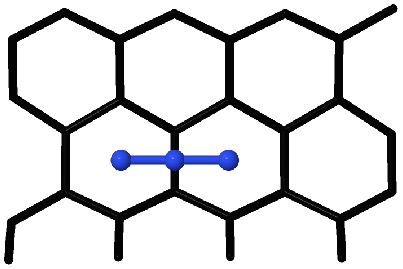
\includegraphics[width=\textwidth]{n3_t553_start_b-cropped.pdf}
        \caption{bond}
    \end{subfigure}
    \hspace{1cm}
    \begin{subfigure}{3cm}
        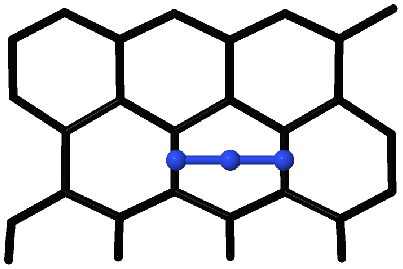
\includegraphics[width=\textwidth]{n3_t553_start_h-cropped.pdf}
        \caption{hollow}
    \end{subfigure}
    \hspace{1cm}
    \begin{subfigure}{3cm}
        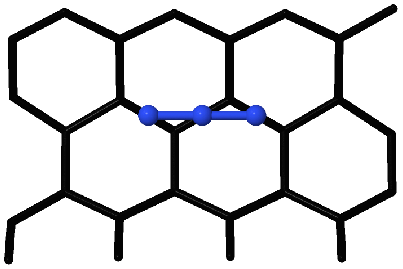
\includegraphics[width=\textwidth]{n3_t553_start_z-cropped.pdf}
        \caption{zigzag}
    \end{subfigure}
    \caption{Starting sites of the bond, hollow and zigzag geometries, respectively.}
}

\bfig{fig:n3t553_start_center}{
    \centering
    \begin{subfigure}{3cm}
        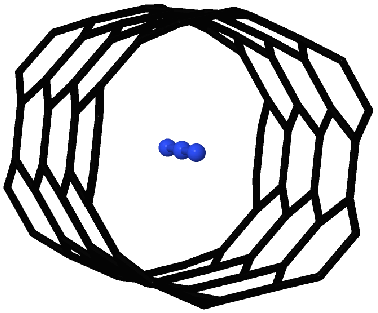
\includegraphics[width=\textwidth]{n3_t553_start_c-cropped.pdf}
    \end{subfigure}
    \hspace{1cm}
    \begin{subfigure}{3cm}
        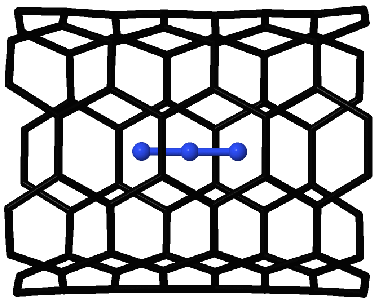
\includegraphics[width=\textwidth]{n3_t553_start_c_side-cropped.pdf}
    \end{subfigure}
    \caption{Central starting geometry (c). Note that the nanotube model has dangling hydrogen atoms at the two ends which are not shown here.}
}

\bfig{fig:n3t553_geom_parms}{
    \centering
    \begin{subfigure}{4.7cm}
        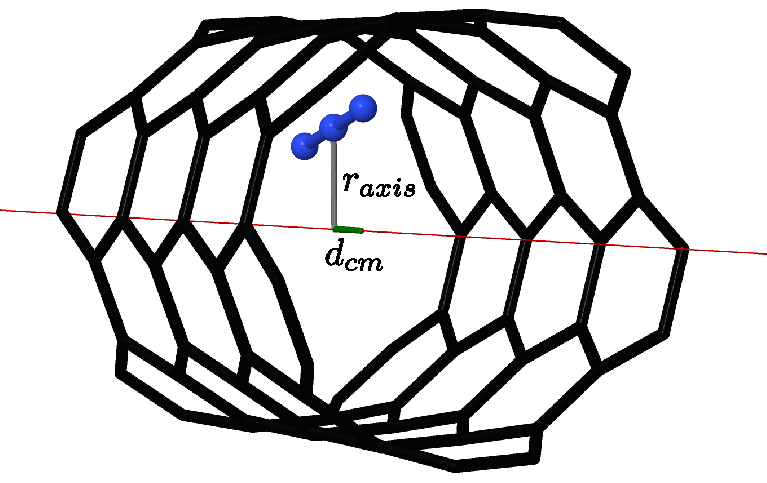
\includegraphics[width=\textwidth]{n3_t553_dist-cropped.pdf}
    \end{subfigure}
    \hspace{1cm}
    \begin{subfigure}{4cm}
        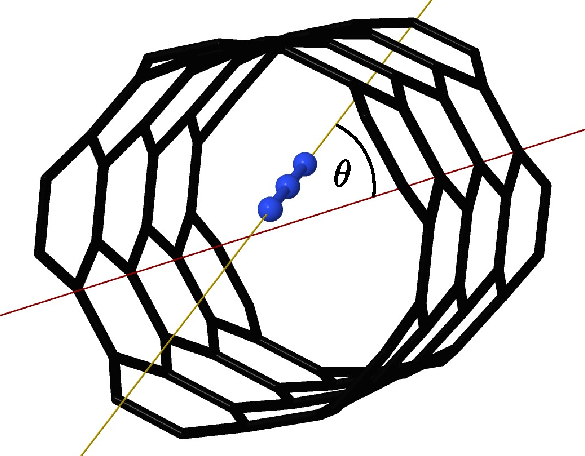
\includegraphics[width=\textwidth]{n3_t553_angle-cropped.pdf}
    \end{subfigure}
    \caption{Geometrical parameters.}
}

\def\btab#1#2{\expandafter\gdef\csname tab-#1\endcsname{\begin{table}[ht]#2\label{#1}\end{table}}}
\def\tref#1{\csname tab-#1\endcsname\Cref{#1}}

\btab{tab:geom_comp}{
    \centering
    \begin{tabular}{crrrrr}
        \toprule
        \textit{$\Lambda$} & site & $d_{cm}$ (\AA) & $r_{axis}$ (\AA) & $\theta$ ($^{\circ}$) & $\Delta E_{int}$ (kcal/mol) \\
        \midrule
        \multirow{3}{*}{3} & \textit{bond} & $ 0.018$ & $ 0.002$ & $0.06$ & $-0.001$ \\
        ~ & \textit{hollow}                & $ 0.002$ & $ 0.003$ & $0.04$ & $ 0.000$ \\
        ~ & \textit{zigzag}                & $ 0.000$ & $ 0.003$ & $0.27$ & $-0.002$ \\
        \midrule
        \multirow{3}{*}{5} & \textit{bond} & $ 0.604$ & $ 0.009$ & $0.32$ & $ 0.112$ \\
        ~ & \textit{hollow}                & $-0.144$ & $ 0.002$ & $0.32$ & $ 0.017$ \\
        ~ & \textit{zigzag}                & $ 0.000$ & $ 0.003$ & $0.43$ & $ 0.000$ \\
        \midrule
        \multirow{3}{*}{7} & \textit{bond} & $ 0.470$ & $ 0.029$ & $1.10$ & $ 0.588$ \\
        ~ & \textit{hollow}                & $-0.233$ & $ 0.027$ & $0.54$ & $ 0.417$ \\
        ~ & \textit{zigzag}                & $ 0.001$ & $ 0.038$ & $0.18$ & $ 0.363$ \\
        \midrule
        \multirow{3}{*}{9} & \textit{bond} & $ 0.622$ & $ 0.015$ & $0.74$ & $ 0.400$ \\
        ~ & \textit{hollow}                & $-1.304$ & $ 0.003$ & $0.17$ & $ 0.030$ \\
        ~ & \textit{zigzag}                & $-0.007$ & $ 0.004$ & $0.53$ & $ 0.141$ \\
        \bottomrule
    \end{tabular}
    \caption{Geometrical parameters and interaction energy difference with respect to the (c) geometry. Note that the $d_{cm}$, $r_{axis}$ and $\theta$ are all zero for the (c) geometry.}
}

\btab{tab:eint_cnt55x_cc-pvtz}{
    \centering
    \begin{tabular}{r cccccc}
        \toprule
        $\Lambda$-CNT & 3-CNT     & 5-CNT     & 7-CNT     & 9-CNT    & 11-CNT   & 13-CNT   \\
        occ./virt.    & 260/2800  & 380/4000  & 500/5200  & 620/6400 & 740/7600 & 860/8800 \\
        \midrule
        RI-B97D3      & $-30.80$  & $-38.29$  & $-42.58$  & $-45.73$ & $-48.06$ & $-49.94$ \\
        \textit{Time} & 27m       & 50m       & 1h20m     & 2h20m    & 4h12m    & 7h35m    \\
        \vspace{1mm} \\
        RI-SCS-MP2    & $-34.56$  & $-43.36$  & $-$       & $-$      & $-$      & $-$ \\
        \textit{Time} & 8h        & 36h (8cpus) & $-$     & $-$      & $-$      & $-$ \\
        \bottomrule
    \end{tabular}
    \caption{CP-corrected unrelaxed interaction energies of N$_3^-$ confined inside a $(5,5)$ SWCNT of increasing length. The azide anion is placed perfectly in the center of the nanotube, parallel to the principal axis. The basis set use is the \textbf{cc-pvtz} with the addition of diffuse functions (aug-) on the anion. All energies are given in kcal/mol.}
}

\btab{tab:eint_cnt55x_cc-pvdtz}{
    \centering
    \begin{tabular}{r cccccc}
        \toprule
        $\Lambda$-CNT & 3-CNT     & 5-CNT     & 7-CNT     & 9-CNT    & 11-CNT   & 13-CNT   \\
        occ./virt.    & 260/1400  & 380/1900  & 500/2500  & 620/3000 & 740/3600 & 860/4150 \\
        \midrule
        RI-B97D3      & $-26.26$  & $-33.97$  & $-38.50$  & $-41.85$ & $-44.36$ & $-46.36$ \\
        \textit{Time} & 9m        & 20m       & 33m       & 45m      & 62m      & 1h25m    \\
        \vspace{1mm} \\
        RI-SCS-MP2    & $-29.77$  & $-38.87$  & $-43.58$  & $-47.07$ & $-49.88$ & $-$ \\
        \textit{Time} & 1h40m     & 6h        & 10h       & 24h      & 50h20m   & $-$ \\
        \vspace{1mm} \\
        DLPNO-CCSD(T) & $-31.96$  & $-$       & $-$       & $-$      & $-$      & $-$ \\
        \textit{Time} & 28h       & $-$       & $-$       & $-$      & $-$      & $-$ \\
        \bottomrule
    \end{tabular}
    \caption{CP-corrected unrelaxed interaction energies of N$_3^-$ confined inside a $(5,5)$ SWCNT of increasing length. The azide anion is placed perfectly in the center of the nanotube, parallel to the principal axis. The basis set use is the \textbf{cc-pvdz} on the nanotube and the aug-cc-pvtz on the anion. All energies are given in kcal/mol.}
}

\btab{tab:ILJ_parms}{
    \centering
    \begin{tabular}{l cccc}
        \toprule
        atom types      & $\epsilon$  & $r_0$     & $\beta$ & $m$ \\
        \midrule
        C--N$_{1,3}$     & 5.205       & 3.994     & 6--9    & 6.0 \\
        C--N$_{2}$       & 3.536       & 3.828     & 6--9    & 6.0 \\
        \bottomrule
    \end{tabular}
    \caption{ILJ parameters for the interaction of N$_{3}^{-}$ confined inside a carbon nanotube. Different values of $\beta$ are tested.}
}

\btab{tab:n3_t553_ILJ_eint}{
    \centering
    \begin{tabular}{l rrr}
        \toprule
        Terms                & $\beta = 7.0$ & $\beta = 8.0$ & $\beta = 9.0$ \\
        \midrule
        $V_{ILJ}$ [kcal/mol] & $-10.90$      & $-9.68$       & $-8.37$      \\
        $V_{els}$ [kcal/mol] & $+42.24$      & $+42.24$      & $+42.24$      \\
        $V_{ind}$ [kcal/mol] & $-52.91$      & $-52.91$      & $-52.91$      \\
        \midrule
        $V_{tot}$ [kcal/mol] & $-21.57$      & $-20.35$      & $-19.04$      \\
        \midrule
        $V_{SCS-MP2/DZP}$ [kcal/mol]       & \multicolumn{3}{c}{$-26.94$}  \\
        $V_{SCS-MP2/TZP}$ [kcal/mol]       & \multicolumn{3}{c}{$-34.52$}  \\
        $V_{L-CCSD(T)/DZP}$ [kcal/mol]       & \multicolumn{3}{c}{$-28.84$} \\
        $\bar{V}_{L-CCSD(T)/TZP}$ [kcal/mol] & \multicolumn{3}{c}{$-36.42$} \\
        \bottomrule
    \end{tabular}
    \caption{Interaction energies for N$_3^-$ confined inside a 3-CNT(5,5).}
}

\btab{tab:n3_t555_ILJ_eint}{
    \centering
    \begin{tabular}{l rrr}
        \toprule
        Terms                & $\beta = 7.0$ & $\beta = 8.0$ & $\beta = 9.0$ \\
        \midrule
        $V_{ILJ}$ [kcal/mol] & $-12.33$      & $-11.15$      & $-9.89$       \\
        $V_{els}$ [kcal/mol] & $+27.55$      & $+27.55$      & $+27.55$      \\
        $V_{ind}$ [kcal/mol] & $-56.83$      & $-56.83$      & $-56.83$      \\
        \midrule
        $V_{tot}$ [kcal/mol] & $-41.61$      & $-40.43$      & $-39.16$      \\
        \midrule
        $V_{SCS-MP2/DZP}$ [kcal/mol]       & \multicolumn{3}{c}{$-36.06$}  \\
        $V_{SCS-MP2/TZP}$ [kcal/mol]       & \multicolumn{3}{c}{$-43.36$}  \\
        $V_{L-CCSD(T)/DZP}$ [kcal/mol]       & \multicolumn{3}{c}{$-37.08$} \\
        $\bar{V}_{L-CCSD(T)/TZP}$ [kcal/mol] & \multicolumn{3}{c}{$-44.34$} \\
        \bottomrule
    \end{tabular}
    \caption{Interaction energies for N$_3^-$ confined inside a 5-CNT(5,5).}
}

\btab{tab:n3_t557_ILJ_eint}{
    \centering
    \begin{tabular}{l rrr}
        \toprule
        Terms                & $\beta = 7.0$ & $\beta = 8.0$ & $\beta = 9.0$ \\
        \midrule
        $V_{ILJ}$ [kcal/mol] & $-12.79$      & $-11.66$      & $-10.46$      \\
        $V_{els}$ [kcal/mol] & $+18.70$      & $+18.70$      & $+18.70$      \\
        $V_{ind}$ [kcal/mol] & $-57.71$      & $-57.71$      & $-57.71$      \\
        \midrule
        $V_{tot}$ [kcal/mol] & $-51.81$      & $-50.68$      & $-49.48$      \\
        \midrule
        $V_{SCS-MP2/DZP}$ [kcal/mol]       & \multicolumn{3}{c}{$-40.81$}  \\
        $V_{SCS-MP2/TZP}$ [kcal/mol]       & \multicolumn{3}{c}{$-47.84$}  \\
        $V_{L-CCSD(T)/DZP}$ [kcal/mol]       & \multicolumn{3}{c}{$-41.91$}  \\
        $\bar{V}_{L-CCSD(T)/TZP}$ [kcal/mol] & \multicolumn{3}{c}{$-48.94$}  \\
        \bottomrule
    \end{tabular}
    \caption{Interaction energies for N$_3^-$ confined inside a 7-CNT(5,5).}
}

\btab{tab:n3_t559_ILJ_eint}{
    \centering
    \begin{tabular}{l rrr}
        \toprule
        Terms                & $\beta = 7.0$ & $\beta = 8.0$ & $\beta = 9.0$ \\
        \midrule
        $V_{ILJ}$ [kcal/mol] & $-12.73$      & $-11.58$      & $-10.37$      \\
        $V_{els}$ [kcal/mol] & $+13.64$      & $+13.64$      & $+13.64$      \\
        $V_{ind}$ [kcal/mol] & $-58.27$      & $-58.27$      & $-58.27$      \\
        \midrule
        $V_{tot}$ [kcal/mol] & $-57.36$      & $-56.22$      & $-55.00$      \\
        \midrule
        $V_{SCS-MP2/DZP}$ [kcal/mol] & \multicolumn{3}{c}{$-44.31$}  \\
        \bottomrule
    \end{tabular}
    \caption{Interaction energies for N$_3^-$ confined inside a 9-CNT(5,5).}
}

\btab{tab:n3_t5511_ILJ_eint}{
    \centering
    \begin{tabular}{l rrr}
        \toprule
        Terms                & $\beta = 7.0$ & $\beta = 8.0$ & $\beta = 9.0$ \\
        \midrule
        $V_{ILJ}$ [kcal/mol] & $-12.67$      & $-11.52$      & $-10.28$      \\
        $V_{els}$ [kcal/mol] & $+10.60$      & $+10.60$      & $+10.60$      \\
        $V_{ind}$ [kcal/mol] & $-58.54$      & $-58.54$      & $-58.54$      \\
        \midrule
        $V_{tot}$ [kcal/mol] & $-60.61$      & $-59.46$      & $-58.23$      \\
        \midrule
        $V_{SCS-MP2/DZP}$ [kcal/mol] & \multicolumn{3}{c}{$-47.12$}  \\
        \bottomrule
    \end{tabular}
    \caption{Interaction energies for N$_3^-$ confined inside a 11-CNT(5,5).}
}

\btab{tab:n3_t5513_ILJ_eint}{
    \centering
    \begin{tabular}{l rrr}
        \toprule
        Terms                & $\beta = 7.0$ & $\beta = 8.0$ & $\beta = 9.0$ \\
        \midrule
        $V_{ILJ}$ [kcal/mol] & $-$      & $-$      & $-$      \\
        $V_{els}$ [kcal/mol] & $-$      & $-$      & $-$      \\
        $V_{ind}$ [kcal/mol] & $-$      & $-$      & $-$      \\
        \midrule
        $V_{tot}$ [kcal/mol] & $-$      & $-$      & $-$      \\
        \midrule
        $V_{SCS-MP2/DZP}$ [kcal/mol] & \multicolumn{3}{c}{$-49.16$}  \\
        \bottomrule
    \end{tabular}
    \caption{Interaction energies for N$_3^-$ confined inside a 11-CNT(5,5).}
}

\btab{tab:n3_t553_dft_comp}{
    \centering
    \scriptsize
    \begin{tabular}{cccccccc}
        \toprule
        SCS-MP2 & B97-D3  & BLYP-D3 & rPW86PBE-D3 & wB97X-D3 & TPSS0-D3 & B3LYP-D3 & PW6B95-D3  \\
        \midrule
        $-2.19$ & $-5.70$ & $-4.99$ & $-6.89$     & $-6.28$  & $-8.08$  & $-6.88$  & \\
        \bottomrule
    \end{tabular}
    \caption{Interaction energy differences in kcal/mol of various density functionals with respect to the reference DLPNO-CCSD(T) value for N$_3^-$ confined inside a 3-CNT(5,5).}
}

\btab{tab:els_basis_comp}{
    \centering
    \begin{tabular}{c ccc}
        \toprule
        $\Lambda$ & cc-pvdz & cc-pvtz & cc-pvqz \\
        \midrule
        3         & $48.20$ & $42.24$ & $45.20$ \\
        5         & $31.46$ & $27.55$ & $28.78$ \\
        \bottomrule
    \end{tabular}
    \caption{Comparison of electrostatic contribution in kcal/mol with respect to the basis set used in the calculation to obtain the partial atomic charges.}
}


%
% A second series of test has been done by resetting the term $\tfrac{n_2}{n_2 - 4}$, which depends on $\beta$ and therefore will change accordingly.
% \Cref{tab:eint_geo_1_ind_beta} shows the results in this case.
% %
% \begin{table}
%     \centering
%     \begin{tabular}{l|rrrr}
%         $E_{int}$            & $\beta = 6.0$ & $\beta = 7.0$ & $\beta = 8.0$ & $\beta = 9.0$ \\
%         \midrule
%         $V_{ILJ}$ [meV]      &  -569.17      &  -517.63      &  -462.66      &  -403.66      \\
%         $V_{ILJ}$ [kcal/mol] &   -13.12      &   -11.94      &   -10.67      &    -9.31      \\
%         $V_{ind}$ [meV]      & -4033.24      & -3818.14      & -3657.00      & -3531.54      \\
%         $V_{ind}$ [kcal/mol] &   -93.01      &   -88.05      &   -84.33      &   -81.44      \\
%         \midrule
%         $E_{int}$ [meV]      & -4602.40      & -4335.77      & -4119.67      & -3935.20      \\
%         $E_{int}$ [kcal/mol] &  -106.13      &   -99.98      &   -95.00      &   -90.75
%     \end{tabular}
%     \caption{Interaction energies computed using ILJ and the induction term for different $\beta$ values. The term $\tfrac{n_2}{n_2 - 4}$ in the induction potential was let free to vary. The reference MP2 value is -32.31 kcal/mol (-1401.13 meV).}
%     \label{tab:eint_geo_1_ind_beta}
% \end{table}
% %
% A third series of calculations has been performed using NBO charges calculated on the MP2 density; namely $q_1 = q_3 = -0.51$ and $q_2 = -0.01$. Note that the total charge on the trinitrogen anion is not exactly $-1$, but a tiny donation from the nanotube to the confined molecule has occurred. The results for this charge distributions are not listed because for both cases considered above, the resulting interaction energies are constantly lower (i.e. more favorable) by about 4 to 6 kcal/mol.


\title{\LARGE Static and Dynamics of the Azide Anion Confined in an Armchair Carbon Nanotube}

\author{Stefano Battaglia}

\begin{document}

\maketitle

\section{Introduction}
Introduction

\section{Computational Details}
The computational details section is divided in two parts.
The first one describes the details of the \textit{ab-initio} calculations performed in order to obtain accurate interaction energies and partial atomic charges of the two fragments.
The second one describes the analytical potential employed in the molecular dynamics (MD) simulations and assesses its performance against the \textit{ab-initio} values.


\subsection{\textit{Ab-Initio}}
At \textit{ab-initio} level, carbon nanotubes (CNTs) have been treated as finite-size systems and the two open ends have been capped with hydrogen atoms in order to fill out the valence shell. Only one type of armchair nanotube has been considered, with chiral indices $(5,5)$. In order to obtain converged values with respect to the length of the nanotube, CNTs with different number of units have been studied. We introduce here the notation $\Lambda$-$(5,5)$CNT to label a nanotube composed by $\Lambda$ units, where a single unit corresponds to a [$10$]cyclophenacene (see FIGURE).


\subsubsection{Geometries}
The geometries of the nanotubes and the azide anion have been optimized using restricted Kohn-Sham density functional theory (DFT), employing the B97D3 exchange-correlation functional with Becke-Johnson damping\cite{Grimme2010,Grimme2011}.
For both fragments Dunning's triple-$\zeta$ cc-pVTZ basis set\cite{DunningJr1989} has been used, with the addition of diffuse functions (aug-)\cite{Kendall1992} in the case of the \ntm fragment.\\
The nanotubes geometries retained the high $D_{5d}$ symmetry, with both parallel and perpendicular (to the principal axis) C--C bonds showing the typical alternation pattern of these systems when treated with open boundary conditions\cite{Zhou2004,Galano2006}. As the length of the nanotube increases, the average C--C bond length also increases, from $1.4237$ \AA\ to $1.4268$ \AA, which is in agreement with the fact that the bond gets slightly stretched due to the curvature.\\
The relaxed \ntm geometry has linear $D_{\infty h}$ symmetry, with an N--N bond length of $1.1874$ \AA, which is in excellent agreement with the experimental gas phase value of $1.1884$ \AA\cite{Polak1987}.\\
All the optimizations just mentioned have been performed using the Gaussian 09 software package, revision d01\cite{g09}, using the default convergence thresholds, the ultrafine grid for the integral quadrature and spherical \textit{d} and \textit{f} basis functions.


\subsubsection{Interaction Energies}
In order to construct the classical force field (cf. Molecular Dynamics section), the most important parameter to obtain is the interaction energy of the the guest \ntm ion and the host carbon nanotube at the optimal adsorption distance.
In this contribution, all interaction energies computed using first principles methods have been evaluated according to the formula
%
\begin{equation}
    E_{int} = E_{complex} - (E_{cnt} + E_{azide}) \label{eq:eint}
\end{equation}
%
where the fragment energies $E_{cnt}$ and $E_{azide}$ have been computed in the basis set of the complex system, thus correcting the basis set superposition error according to the Boys and Bernardi scheme\cite{Boys1970}.
Relaxation effects on the two interacting fragments have not been taken into account, although it has been recently shown that they contribute only in the order of 1--2 kcal/mol\cite{Battaglia2017a} to $E_{int}$ and thus do not substantially modify the overall picture.\\
To locate the minimum of the potential energy surface (PES), a series of constrained optimizations involving nanotubes of lengths between 3 and 9 units has been performed. In these optimizations, the optimal geometry of the two fragments has been kept frozen and only their relative distance and orientation have been optimized, thus locating the adsorption distance.
This series of optimizations has been performed using the ORCA 4 program package\cite{ORCA4} at the same level of theory as before, besides employing the smaller cc-pVDZ basis set on the nanotube, the resolution of the identity technique for the Coulomb matrix using the auxiliary basis def2/J by Weigend \textit{et al.}\cite{Weigend2006}.\\
Remarkably, it turns out that in the particular case of an azide anion confined inside a $(5,5)$CNT, the geometry with the \ntm molecule placed exactly in the center of the nanotube, aligned to its principal axis, results to be a local minimum. Moreover, the difference between this minimum and the lowest minimum found is at most less than $0.6$ kcal/mol for the nanotubes studied. For this reason, the geometry with the \ntm molecule placed in the center of the CNTs has been used for the calculation of $E_{int}$ at higher levels of theory and for nanotubes longer than 9 units.
For a detailed explanation of the structure optimizations, the criteria used to compare them and all the geometries, we point the reader to the Supplementary Information.\\

%%%%
As we are dealing with finite size CNTs, it is important to study the dependence of the interaction energy with respect to the length of the nanotube. In particular, given that the confined species is negatively charged, one expects a slower convergence compared to neutral systems due to the typically more diffuse electron density of anions.\\
Accurate interaction energies have been calculated at wave function level of theory, using the density-fitted spin-component-scaled MP2 method (RI-SCS-MP2)[REFERENCE] and the local coupled cluster method DLPNO-CCSD(T) as implemented in the ORCA 4 program package\cite{Riplinger2013,Riplinger2016}. Calculations have been performed using the cc-pVDZ or the cc-pVTZ basis set (where computationally feasible) and in both cases diffuse functions (aug-) have been added on the \ntm species.\\
\fref{fig:n3t55x_ab-initio_eint} depicts the results obtained for nanotubes of different lengths, where it is immediately clear that interaction energy shows a slow convergence rate with respect to $\Lambda$.
In order to obtain accurate interaction energies within a sufficiently large basis set, extrapolated DLPNO-CCSD(T)/cc-pVTZ values have been obtained using the following formula
%
\begin{equation}
    E_{CC}(pVTZ) \approx E_{MP2}(pVTZ) + (E_{CC}(pVDZ) - E_{MP2}(pVDZ)) \label{eq:basis_extr}
\end{equation}
%
where it is assumed that the correlation energy difference between the two methods is constant with respect to the basis set used.
This approach has allowed us to obtain approximate accurate values for nanotubes of length 3, 5 and 7. Nonetheless, as it can be seen from the RI-SCS-MP2/cc-pVDZ curve in \Cref{fig:n3t55x_ab-initio_eint}, $E_{int}$ still significantly decreases with the addition of extra nanotube units.
Therefore, in order to be able to extrapolate the DLPNO-CCSD(T)/cc-pVTZ confinement energy inside an arbitrary $\Lambda$-(5,5) nanotube we use the following formula
%
\begin{equation}
    E_{int}(\Lambda) = \frac{a\Lambda}{b + \Lambda} \label{eq:length_extr}
\end{equation} 
%
where $a$ and $b$ are two fitting parameters to be determined.
\Cref{eq:length_extr} is the simplest formula which satisfies the condition $E_{int}(0) = 0$ and provides an estimate for the infinitely long nanotube through the parameter $a$.\\
The solid lines in \Cref{fig:n3t55x_ab-initio_eint} show the non-linear least square fits to the RI-SCS-MP2/cc-pVDZ and the approximated DLPNO-CCSD(T)/cc-pVTZ interaction energies computed according to \cref{eq:basis_extr}.
The extrapolated value for $E_{int}$ in the limit of an infinitely long CNT is $-65.93$ kcal/mol.
For a detailed explanation of the parameters used in the calculation and the tests performed to assess the validity of our approach, we point the reader to the Supplementary Information.\\


\subsection{Molecular Dynamics}
The Improved Lennard-Jones (ILJ) potential\cite{Pirani2008} is given by
%
\begin{equation}\label{eq:V_ILJ}
    V_{ILJ}(r_{ij}) = \epsilon \left[ \frac{m}{n(r_{ij})-m} \cdot \Big( \frac{r_m}{r_{ij}} \Big)^{n(r_{ij})} -
                                 \frac{n(r_{ij})}{n(r_{ij})-m} \cdot \Big( \frac{r_m}{r_{ij}} \Big)^{m} \right]
\end{equation}
%
where
%
\begin{equation}
    n(r_{ij}) = \beta + 4.0 \cdot \Big( \frac{r_{ij}}{r_m} \Big)^2
\end{equation}
%
and $r_{ij}$ is the distance between atom $i$ in the carbon nanotube and atom $j$ in the \ntm
molecule. The parameters $r_m$ and $\epsilon$ are set according to the atoms interacting,
$\beta$ is a free parameter used to fit the potential to experimental or numerical values,
while $m$ is set according the to the partial charges of the interacting species.
Since the azide anion has a total negative charge of $-1$, one has to introduce a non-bonded term in the potential which accounts for the induced polarization on the carbon nanotube due to the excess negative charge of the anion.
The potential term $V_{ind}$ describing the dipole induced by the $\text{N}_3^-$ anion on a neutral fragment is given by
%
\begin{equation}\label{eq:V_ind}
    V_{ind}(r_{i1},r_{i2},r_{i3}) = - \frac{1}{2} \cdot \alpha \cdot f(r_{i1},r_{i2},r_{i3})
        \left[ \frac{q_1}{r_{i1}^2} + \frac{q_2}{r_{i2}^2} + \frac{q_3}{r_{i3}^2} \right]^2
\end{equation}
%
where $r_{i1}$, $r_{i2}$ and $r_{i3}$ are the distances between atom $i$ of the neutral species and the three nitrogen atoms of the azide anion, $q_1$, $q_2$ and $q_3$ are the partial charges on the nitrogen atoms, $\alpha$ is the polarizability per volume of the atoms in the neutral species and $f(r_{i1},r_{i2},r_{i3})$ is a damping factor.\\  % $f(R_{i,2}) = \frac{n(R_{i,2})}{n(R_{i,2}) - 4}$
By saturating the CNT with hydrogen atoms, the two ends of the nanotube result significantly polarized with partial atomic charges in the range of $\pm 0.2$.
As a consequence, the \ntm interacts through the usual Coulomb potential with the partial atomic charges on the nanotube, giving rise to an additional term $V_{els}$ describing this electrostatic potential as
%
\begin{equation}
    V_{els}(r_{ij}) = \frac{q_i q_j}{r_{ij}}
\end{equation}
%
This \textit{artificial} term vanishes when hydrogen atoms are removed from the nanotube or the nanotube is considered with periodic boundary conditions. This follows from the fact that the partial atomic charge on each carbon atom is equal zero ($q_i \equiv 0$ $\forall i$) and thus $V_{els}(r_{ij}) = 0$.\\

The total interaction energy $E_{int}$ is finally obtained by summing the potential terms just described over all atoms of both fragments as follows
%
\begin{align}
    E_{int} = \sum_{i=1}^{N_C + N_H} V^{(i)}_{ind}(r_{i1},r_{i2},r_{i3}) +
              \sum_{j=1}^{N_N} V_{ILJ}^{(ij)}(r_{ij}) + V_{els}(r_{ij})
\end{align}
%
where $N_C$, $N_N$ and $N_H$ correspond to the total number of carbon, nitrogen and hydrogen atoms, respectively.
The superscript $(ij)$ in the ILJ potential term $V_{ILJ}^{(ij)}$ keeps track of the interacting atom types such that the parameters can be accordingly set to the values given in \tref{tab:ILJ_parms}.
The ILJ parameters have been obtained following the approach illustrated in Ref. \citenum{Cambi1991}, which is based on the static atomic dipole polarizabilities of the interacting fragments.
For hydrogen and carbon, the polarizabilities were taken from Refs. \citenum{Gavezzotti2003} and \citenum{Torrens2004}, while for nitrogen, the \ntm experimental total mean polarizability\cite{Borgne1999}, $\bar{\alpha} = 4.65$ \AA$^3$, has been distributed on the three atoms according to their partial charges.
All values are listed in \tref{tab:polarizabilities}.
The partial atomic charges on the azide anion were set to be $q_1 = q_3 = -0.56$ and $q_2 = 0.12$, while for the carbon nanotube they have been obtained through a natural population analysis\cite{Reed1985a} of the electron density calculated at B97D3/cc-pVTZ level of theory.\\
Additional information on the atomic polarizabilities and the procedure used to obtain the ILJ parameters is available in the Supplementary Information.\\

In \fref{fig:n3t55x_comp_eint} it can be seen the direct comparison of the \emph{ab-initio} and the classical potential ($\beta = 8$ and $f(r_{i1},r_{i2},r_{i3}) = 1$) for nanotubes with $\Lambda = 3,5,7,9,11,13$. 
The various components of the classical potential can also be considered separately, and these are listed in \tref{tab:pot_comp} and plotted in \fref{fig:n3t55x_classical_eint} along with the total and the \emph{ab-initio} ones.

\clearpage

\bibliographystyle{unsrt}
\bibliography{library}

\clearpage
\section{Supplementary Information}

\subsection{Geometry Optimization}
To ensure that the relaxation process did not remain trapped in a local minimum and without knowing a priori the optimal adsorption distance of the \ntm molecule, the optimization procedure has been started from four different geometries.
In all cases, the anion has been placed parallel to the principal axis of the nanotube.
Three starting geometries were chosen according to possible adsorption sites in which the central nitrogen atom of the azide was placed either over C--C bonds (\textit{bond} (b) and \textit{zigzag} (z) geometries) or in the center of an hexagonal ring of the CNT wall (\textit{hollow} (h) geometry). The three starting sites are shown in \fref{fig:n3t553_start_sites}, along with their labels that will be used in the following to refer to them. For all three cases, the azide anion has been placed at a distance of about $2.25$\AA\ from the nanotube wall.
The fourth starting geometry is shown in \fref{fig:n3t553_start_center} and it simply consists in the \ntm anion placed exactly in the center of the nanotube. We will refer to this starting geometry as \textit{central} (c) geometry.
In order to study the edge effects on the position of the minimum, CNTs of four different lengths have been considered, namely with 3, 5, 7 and 9 units.
The relaxed structures starting from the (c) geometry correspond to a (local) minimum, since after one optimization step the convergence is reached, with the \ntm anion insignificantly ($\approx 0.002$\AA) shifted out of the principal axis. For this reason we will consider from now on the (c) geometry as the perfectly aligned anion to the principal axis and sitting in the center of the nanotube.
For the three other starting conformations, namely the the (b), (h) and (z) geometries, the relaxation leads to different (local) minima.
In order to analyze the differences in the final structures, three geometrical parameters and an energetic one have been considered.
The geometrical parameters are depicted in \fref{fig:n3t553_geom_parms} and consist in the axial distance $d_{cm}$ between the center of mass of the azide anion and the center of mass of the carbon nanotube, the radial distance $r_{axis}$ of the azide anion center of mass from the principal axis of the nanotube and the angle $\theta$ formed between the principal axis and an imaginary line passing through the external nitrogen atoms of the azide anion.
The energetic parameter is the interaction energy $E_{int}$ between the two fragments, computed according to \Cref{eq:eint}.\\
The geometrical parameters computed for all systems are listed in \tref{tab:geom_comp}. Since the (c) geometry consists in the azide ion sitting in the exact center of the nanotube, the three conformational parameters are all zero in that case, thus for geometries (b), (h) and (z), the parameters can be considered as deviations from the (c) geometry. Accordingly, instead of tabulating the interaction energy for every geometry, the values listed in the last column of \Cref{tab:geom_comp} correspond to the interaction energy difference between the (c) geometry and the other three, i.e. $\Delta E_{int} = E_{int}(c) - E_{int}(site)$. A negative value for $\Delta E_{int}$ means that the interaction energy is more favorable (i.e. stronger) for the (c) geometry, while a positive value the opposite.\\
For all final geometries, the azide anion is found to be almost perfectly aligned to the principal axis of the nanotube since the angle $\theta$ is always very small (below $1^{\circ}$ except in one case).
Similarly, $r_{axis}$ is also always particularly small (most of the times below $0.01$ \AA), meaning that the anion has the preference to stay approximately at the same distance from the nanotube wall in all directions.
In particular, irrespective of the length $\Lambda$, the azide ion is adsorbed at a distance of approximately $3.34$ \AA\ (computed as the distance between the \ntm center of mass and the closest side of the wall). This value is significantly larger than the adsorption distance of $3.17$ \AA\ found for the confinement in a larger 3-CNT(6,6), obtained following the same computational procedure.\\
There are two possible explanations for the difference in the adsorption distance. Either the different curvature of the two nanotubes is such that the forces attracting the ion are stronger in the case of the (6,6) CNT, or, in the case of the (5,5) CNT, there is a competition between the attractive forces exerted by the surrounding wall on the azide ion, which eventually stabilizes it at an (almost) equal radial distance in any direction.
The analysis of the curvature effects on the adsorption distance inside the CNT are beyond the scope of this work, and thus not further investigated here.\\
The most fluctuating parameter is $d_{cm}$. Clearly, the periodic atomic pattern of the carbon nanotube makes the potential energy surface (PES) of the complex full of local minima, all of which approximately share the same well depth. Apart from the (z) conformation, for which $d_{cm}$ remains virtually unchanged irrespective of the length, it is hard to rationalize the results for the (b) and (h) cases.
The only exception is found for the 3-CNT(5,5), where the two open ends of the nanotube are so close to the \ntm molecule that the energy barriers to move away from the center are particularly steep and thus confine the azide anion in the center.\\
Nonetheless, although the evident differences between the final geometries, the effects observed on the interaction energy, which is our first and most important parameter, is minimal and most importantly, below chemical accuracy ($\approx 1$ kcal/mol).
As it appears a very hard task to find the \emph{global minimum} for this type of systems and considering the small influence observed on the interaction energy, the central geometry (c) has been used for all interaction energies computed in this work.

\subsection{Interaction Energies}
The parameters obtained through the non-linear least square fits of the RI-SCS-MP2/cc-pVDZ and the approximated DLPNO-CCSD(T)/cc-pVTZ interaction energies are given in \tref{tab:fit_eint}.

Interaction energies have been computed at different levels of theory for the shortest nanotubes and using the B97D3 functional for all the lengths considered in this work. A comprehensive summary of the values obtained can be seen in \tref{tab:all_eint}.\\
The RI-MP2 and DLPNO-MP2 values are used as a reference to check the error introduced by the DLPNO methods.
The suggested threshold[REFERENCE] to obtain very accurate results for non-covalently bounded systems is the ``TightPNO''. Nonetheless, the DLPNO-MP2 interaction energies obtained with the ``NormalPNO'' threshold only show small deviations from the canonical RI-MP2 values. For this reason and considering our computational limitations, the DLPNO-CCSD(T) have also been performed using the ``NormalPNO'' threshold.
We argue that the error introduced by the looser cutoffs is anyway smaller than the error introduced with the classical potential.

\subsection{Implementation of Analytical Forces, Virial and Stress Tensor}

\subsubsection{Improved Lennard-Jones Potential}
In the main text, the analytical form of the ILJ potential is presented in \Cref{eq:V_ILJ}.
In order to perform efficiently molecular dynamics simulations, it is required to obtain
and implement in the computer program the expression for calculation the forces acting
on each interaction center due to the potential energy function.\\
We start by labeling the various parts of the ILJ potential as follows
%
\begin{align}
    V_{ILJ}(r_{ij}) &= \epsilon \left[ \frac{m}{n(r_{ij})-m} \cdot
                       \Big( \frac{r_m}{r_{ij}} \Big)^{n(r_{ij})} -
                       \frac{n(r_{ij})}{n(r_{ij})-m} \cdot 
                       \Big( \frac{r_m}{r_{ij}} \Big)^{m} \right] \\
                    &= \epsilon \left[ f(r_{ij}) g(r_{ij}) - h(r_{ij}) j(r_{ij}) \right]
                    \label{eq:V_ILJ_simple}
\end{align}
%
For the implementation of the forces due to a general pairwise potential $V(r)$ in the DL POLY
4 program\cite{}, we are seeking the following intermediate function
%
\begin{equation}
    G(r_{ij}) = - \frac{1}{r_{ij}} \frac{\partial}{\partial r_{ij}} V(r_{ij})
\end{equation}
%
where we kept the notation $G(r_{ij})$, although it has nothing to do with the function
$g(r_{ij})$ appearing in \Cref{eq:V_ILJ_simple}.
The forces on atom $i$ are then evaluated through the following multiplication
%
\begin{equation}\label{eq:forces}
    \begin{aligned}
    \vec{F}_i(r_{ij}) &= G(r_{ij}) \vec{r}_{ij} \\
    &= -\frac{1}{r_{ij}} \left[ \frac{\partial}{\partial r_{ij}} V(r_{ij}) \right] \vec{r}_{ij}
    \end{aligned}
\end{equation}
For the sake of lightening the syntax, in the following derivations we will denote
$r \equiv r_{ij}$.\\
To begin with, let us compute the derivative of the function $n(r)$ appearing in the
potential
%
\begin{align}
    \ddr n(r) &= \ddr \left[ \beta + 4 \left( \frac{r}{r_m} \right)^2 \right] \\
    &= 8 \frac{r}{r_m^2}
\end{align}
%
Next, the derivative of the ILJ potential with respect to $r$ is given, in the simplified
version introduced above, by
%
\begin{equation}\label{eq:dVdr_ILJ_simple}
    \ddr V_{ILJ}(r) = \epsilon \left[ f'(r)g(r) + f(r)g'(r) -
                                      h'(r)j(r) - h(r)j'(r) \right]
\end{equation}
%
where the prime signs indicate a derivative with respect to $r$.
The derivative of $f(r)$ is straightforward and has the following form
%
\begin{equation}
    \ddr f(r) = \ddr\frac{m}{n(r)-m} = n'(r)\frac{-m}{(n(r)-m)^2} = \frac{-n'(r)}{(n(r)-m)}f(r)
\end{equation}
%
The derivative of $g(r)$ is more complicated since $n(r)$ appears in the exponent. Therefore,
we employ the logarithmic differentiation as follows
%
\begin{align}
    \ln (g(r)) &= \ln \left( \frac{r_m}{r} \right) n(r) \\
    \ddr \ln (g(r)) &= \ddr \left[ \ln \left( \frac{r_m}{r}n(r) \right) \right] \\
    g'(r) \frac{1}{g(r)} &= \frac{-1}{r}n(r) + \ln \left( \frac{r_m}{r}n'(r) \right) \\
    g'(r) = \ddr g(r) &= g(r)\left[\ln\left(\frac{r_m}{r}\right)n'(r) - \frac{n(r)}{r}\right]
\end{align}
To obtain $h'(r)$ we carry out the following steps
%
\begin{align}
    \ddr h(r) &= \ddr \frac{n(r)}{n(r)-m} \\
    &= \frac{n'(r)(n(r)-m)-n(r)n'(r)}{(n(r)-m)^2} \\
    &= \frac{n'(r)n(r) - n'(r)m - n(r)n'(r)}{(n(r)-m)^2} \\
    &= \frac{-n'(r)m}{(n(r)-m)^2} \\
    &= \frac{m}{n(r)-m} \frac{-n'(r)}{n(r)-m}
\end{align}
%
Finally, the last derivative reads
%
\begin{equation}
    \ddr j(r) = \ddr \left(\frac{r_m}{r}\right)^m = -m\frac{r_m^m}{r^{m+1}} = \frac{-m}{r}j(r)
\end{equation}
%
By explicitly inserting all the computed terms into \Cref{eq:dVdr_ILJ_simple} we obtain
the final form for $\ddr V_{ILJ}$
%
\begin{align}
    \frac{\partial V_{ILJ}(r)}{\partial r} &= \epsilon
        \left[ f'(r)g(r) + f(r)g'(r) - h'(r)j(r) - h(r)j'(r) \right] \\
    &= \epsilon \left[ 
        t_1 t_2 t_3
        + t_2 t_3 \left[ \ln \left(\frac{r_m}{r}\right)n'(r) - \frac{n(r)}{r} \right]
        - t_1 t_2 t_4
        - \frac{n(r)}{n(r)-m} \frac{-m}{r} t_4 \right]
\end{align}
%
where we have introduced intermediates $t_1, t_2, t_3$ and $t_4$, according to
%
\begin{align}
    t_1 &= \frac{-n'(r)}{n(r)-m} \\
    t_2 &= \frac{m}{n(r)-m} \\
    t_3 &= \left( \frac{r_m}{r} \right)^{n(r)} \\
    t_4 &= \left( \frac{r_m}{r} \right)^m
\end{align}
%
The ILJ force vectors can now be simply computed through \Cref{eq:forces}.\\
Note that the ILJ potential is completely general and can be used with any molecular
species as long as the parameters are accordingly defined.

\subsubsection{Induction Potential}
The induction potential generated by three point charges is defined in \Cref{eq:V_ind}.
In the following we are going to expand the squared term on the right hand side of
\Cref{eq:V_ind} and introduce a more convenient notation for the derivation of the forces,
%
\begin{equation}\label{eq:V_ind_simple}
    \begin{aligned}
        V_{ind}(r_{i1},r_{i2},r_{i3}) &= - \frac{1}{2} \alpha \left[ 
            \frac{q_1}{r_{i1}^2} + \frac{q_2}{r_{i2}^2} + \frac{q_3}{r_{i3}^2} \right]^2 \\
            &= - \frac{1}{2} \alpha \left[ \frac{q_1^2}{r_{i1}^4} + \frac{q_2^2}{r_{i2}^4}
            + \frac{q_3^2}{r_{i3}^4} + \frac{2q_1 q_2}{r_{i1}^2 r_{i2}^2}
            + \frac{2q_2 q_3}{r_{i2}^2 r_{i3}^2} + \frac{2q_1 q_3}{r_{i1}^2 r_{i3}^2} \right] \\
            &= - \frac{1}{2} \alpha \left[ t^i_{11} + t^i_{22} + t^i_{33}
            + 2t^i_{12} + 2t^i_{23} + 2t^i_{13} \right]
    \end{aligned}
\end{equation}
%
where we note that the terms $t^i_{jk} = t^i_{kj}$ are symmetric.\\
As before, we are interested in obtaining all the components of the force vector $\vec{F}_i$
acting on atom $i$. In order to do so, we can differentiate the potential with respect to the
individual components of the coordinate vector $\vec{r}_i = [x_i, y_i, z_i]$.
For example, for the $x$ componet we have
%
\begin{equation}
    \vec{F}_{i,x} = - \dfdx{V_{ind}}{x_i}
\end{equation}
%
and similarly for the other two.\\
The potential $V_{ind}$ depends on the distances $r_{i1}, r_{i2}$ and $r_{i3}$ between
atom $i$ and the three nitrogen atoms, thus to obtain the derivative with respect to the
Cartesian components we have to apply the chain rule, as exemplified in the following for $x_i$
%
\begin{equation}\label{eq:dVdr_ind_simple}
    \dfdx{V_{ind}}{x_i} = \dfdx{V_{ind}}{r_{i1}}\dfdx{r_{i1}}{x_i} +
        \dfdx{V_{ind}}{r_{i2}}\dfdx{r_{i2}}{x_i} + \dfdx{V_{ind}}{r_{i3}}\dfdx{r_{i3}}{x_i}
\end{equation}
%
Let us denote $w_i = \{ x_i,y_i,z_y \}$, then we have in general
%
\begin{equation}
    \dfdx{r_{ij}}{w_i} = \dfdx{}{w_i} \sqrt{(x_i-x_j)^2 + (y_i-y_j)^2 + (z_i-z_j)^2}
        = 2(w_i-w_j) \frac{1}{2} \frac{1}{r_{ij}} = \frac{w_{ij}}{r_{ij}}
\end{equation}
%
where $w_{ij} = w_i - w_j$.\\
The derivatives of the terms $t^i_{jk}$ introduced in \Cref{eq:V_ind_simple} can be
separate into two possible cases.
In the first case, indices $j$ and $k$ are the same
%
\begin{equation}
    \dfdx{t^i_{jj}}{w_i} = \dfdx{t^i_{jj}}{r_{ij}} \dfdx{r_{ij}}{w_i}
        = \dfdx{t^i_{jj}}{r_{ij}} \frac{w_{ij}}{r_{ij}}
        = \left( \dfdx{}{r_{ij}} \frac{q_j^2}{r_{ij}^4} \right) \frac{w_{ij}}{r_{ij}}
        = -4 q_j^2 r_{ij}^{-5} \frac{w_{ij}}{r_{ij}}
        = -4 \frac{q_j^2 w_{ij}}{r_{ij}^6}
\end{equation}
%
In the second case, the indices $j$ and $k$ are different
%
\begin{align}
    \dfdx{t^i_{jk}}{w_i} &= \dfdx{t^i_{jk}}{r_{ij}} \dfdx{r_{ij}}{w_i}
        + \dfdx{t^i_{jk}}{r_{ik}} \dfdx{r_{ik}}{w_i} \\
        &= \dfdx{t^i_{jk}}{r_{ij}} \frac{w_{ij}}{r_{ij}}
        + \dfdx{t^i_{jk}}{r_{ik}} \frac{w_{ik}}{r_{ik}} \\
        &= \left(\dfdx{}{r_{ij}}\frac{q_j q_k}{r_{ij}^2 r_{ik}^2}\right)\frac{w_{ij}}{r_{ij}}
        + \left(\dfdx{}{r_{ik}}\frac{q_j q_k}{r_{ij}^2 r_{ik}^2}\right)\frac{w_{ik}}{r_{ik}} \\
        &= -2 q_j q_k r_{ij}^{-3} r_{ik}^{-2} \frac{w_{ij}}{r_{ij}}
           -2 q_j q_k r_{ij}^{-2} r_{ik}^{-3} \frac{w_{ik}}{r_{ik}} \\
        &= -2 \frac{q_j q_k w_{ij}}{r_{ij}^4 r_{ik}^2}
           -2 \frac{q_j q_k w_{ik}}{r_{ij}^2 r_{ik}^4}
\end{align}
%
The final form of the induction forces can be obtained by inserting all terms just computed
into \Cref{eq:dVdr_ind_simple}, by substituting indices $1,2,3$ with $j$ and $k$.\\
Note that due to the non-additive nature of the induction potential, this derivation
of the forces only applies to the potential generated by three point charges.
Therefore, if more or less charges are the sources of induction, the forces have to be
derived and implemented another time.
Note also that the forces due to the induction potential only apply to atoms not belonging
to \ntm.\\
\\
In order to obtain the pressure of a thermodynamic system, we can rely on Clausis' Virial
theorem, given by
%
\begin{equation}
    P = \frac{1}{3V} \left( 2 \langle K \rangle - \langle \Psi \rangle \right)
\end{equation}
%
where $\langle \Psi \rangle$ is the ensemble average of the virial $\Psi$.\\
Another method to obtain the pressure is by statistical thermodynamics arguments, through
the equation
%
\begin{equation}\label{eq:pressure_td}
    P = -\Bigg< \left( \frac{\partial H^N(\vec{r}^N,\vec{p}^N)}{\partial V} \right)_T\Bigg>
\end{equation}
%
where
%
\begin{equation}\label{eq:Hamiltonian}
    H^N(\vec{r}^N,\vec{p}^N) = K^N(\vec{p}^N) + \Phi^N(\vec{r}^N)
\end{equation}
%
is the Hamiltonian of the system.\\
Note how in \Cref{eq:pressure_td} there is a partial derivative with respect to the system
volume $V$, but in general, the Hamiltonian of \Cref{eq:Hamiltonian} does not contain
the volume explicitly.
In order to introduce the volume and obtain an explicit form of \Cref{eq:Hamiltonian}, we
carry out the following substitution
%
\begin{equation}
    \vec{r}^N = V^{1/3} \vec{s}^N
\end{equation}
%
which introduces the scaled positions $\vec{s}^N$.
After some algebraic manipulation, we obtain the derivative of \Cref{eq:Hamiltonian} w.r.t.
the volume as
%
\begin{align}
    \dfdx{H^N(\vec{r}^N,\vec{p}^N)}{V}&=\dfdx{K^N(\vec{p}^N)}{V}+\dfdx{\Phi^N(\vec{r}^N)}{V} \\
    &= \ldots \\
    &= \frac{-1}{3V} \left( 2K^N(\vec{p}^N) - \Psi^N(\vec{r}^N) \right)
\end{align}
%
which has the same form as Clausius' virial theorem.\\
The virial $\Psi^N(\vec{r}^N)$ is then given by
%
\begin{equation}
    \Psi^N(\vec{r}^N) = \dfdx{\Phi^N(\vec{r}^N)}{\vec{r}^N} \cdot \vec{r}^N
\end{equation}
%
or, alternatively written as
%
\begin{equation}\label{eq:virial}
    \Psi^N(\vec{r}^N) = 3V \dfdx{\Phi^N(\vec{r}^N)}{V}
\end{equation}
%
In order to compute the virial for $V_{ind}$, we use this last equation, after introduction
of the scaled positions in order to have an explicit dependence of the potential w.r.t. the
volume.
The induction potential with scaled positions reads
%
\begin{equation}\label{eq:V_ind_scaled}
    V_{ind}(V^{1/3}s_{i1},V^{1/3}s_{i2},V^{1/3}s_{i3}) = - \frac{1}{2} \alpha \left[
        \frac{q_1}{V^{1/3}s_{i1}^2} + \frac{q_2}{V^{1/3}s_{i2}^2}
        + \frac{q_3}{V^{1/3}s_{i3}^2} \right]^2
\end{equation}
%
By rearranging the terms in \Cref{eq:V_ind_scaled} we have
%
\begin{equation}\label{eq:V_ind_scaled}
    V_{ind}(V^{1/3}s_{i1},V^{1/3}s_{i2},V^{1/3}s_{i3}) = -\frac{1}{2}\alpha\frac{1}{V^{4/3}}
    \left[ \frac{q_1}{V^{1/3}s_{i1}^2} + \frac{q_2}{V^{1/3}s_{i2}^2}
        + \frac{q_3}{V^{1/3}s_{i3}^2} \right]^2
\end{equation}
%
and we can now take the derivative as
%
\begin{align}\label{eq:dVdV_ind}
    \dfdx{V_{ind}}{V} &= \frac{-4}{3} V^{-7/3} \frac{-1}{2} \alpha \left[ 
        \frac{q_1}{s_{i1}^2} + \frac{q_2}{s_{i2}^2} + \frac{q_3}{s_{i3}^2} \right]^2 \\
        &= \frac{-4}{3} V^{-1} \frac{-1}{2} \alpha \left[ V^{-4/3} \left(
        \frac{q_1}{s_{i1}^2} + \frac{q_2}{s_{i2}^2} + \frac{q_3}{s_{i3}^2} \right)^2 \right] \\
        &= \frac{-4}{3V} \frac{-1}{2} \alpha \left[ \frac{q_1}{V^{2/3}s_{i1}^2}
        + \frac{q_2}{V^{2/3}s_{i2}^2} + \frac{q_3}{V^{2/3}s_{i3}^2} \right]^2 \\
        &= \frac{-4}{3V} V_{ind} (r_{i1},r_{i2},r_{i3})
\end{align}
%
By comparing \Cref{eq:dVdV_ind} with \Cref{eq:virial} we see that the virial for particle $i$
due to the induction potential is given by
%
\begin{align}
    \Psi_{ind}^i(r_{i1},r_{i2},r_{i3}) &= 3V \dfdx{V_{ind}}{V} \\
        &= 3V \frac{-4}{3V} V_{ind}(r_{i1},r_{i2},r_{i3}) \\
        &= -4 V_{ind}(r_{i1},r_{i2},r_{i3})
\end{align}
%

\subsection{Implementation Tests}
In this section we show the tests performed in order to validate the implementation of both
the ILJ and the induction potentials.
To perform the tests, we use a simple system that allows us to keep track of all important
quantities, namely a benzene molecule interacting with the \ntm anion as depicted in
\Cref{fig:n3_benzene}.
%
\begin{figure}
    \captionsetup{width=\textwidth}
    \centering
    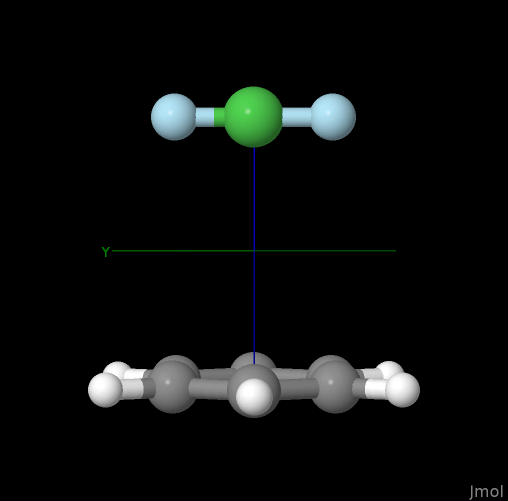
\includegraphics[width=0.5\textwidth]{n3_benzene}
    \caption{Test system.}
    \label{fig:n3_benzene}
\end{figure}
%
The potential energy surface of the \ntm approaching the benzene ring along the $z$-axis
(i.e. the blue line in \Cref{fig:n3_benzene}) is depicted in \Cref{fig:n3_benzene_pes}.
%
\begin{figure}
    \captionsetup{width=\textwidth}
    \centering
    % GNUPLOT: LaTeX picture with Postscript
\begingroup
  \makeatletter
  \providecommand\color[2][]{%
    \GenericError{(gnuplot) \space\space\space\@spaces}{%
      Package color not loaded in conjunction with
      terminal option `colourtext'%
    }{See the gnuplot documentation for explanation.%
    }{Either use 'blacktext' in gnuplot or load the package
      color.sty in LaTeX.}%
    \renewcommand\color[2][]{}%
  }%
  \providecommand\includegraphics[2][]{%
    \GenericError{(gnuplot) \space\space\space\@spaces}{%
      Package graphicx or graphics not loaded%
    }{See the gnuplot documentation for explanation.%
    }{The gnuplot epslatex terminal needs graphicx.sty or graphics.sty.}%
    \renewcommand\includegraphics[2][]{}%
  }%
  \providecommand\rotatebox[2]{#2}%
  \@ifundefined{ifGPcolor}{%
    \newif\ifGPcolor
    \GPcolortrue
  }{}%
  \@ifundefined{ifGPblacktext}{%
    \newif\ifGPblacktext
    \GPblacktexttrue
  }{}%
  % define a \g@addto@macro without @ in the name:
  \let\gplgaddtomacro\g@addto@macro
  % define empty templates for all commands taking text:
  \gdef\gplbacktext{}%
  \gdef\gplfronttext{}%
  \makeatother
  \ifGPblacktext
    % no textcolor at all
    \def\colorrgb#1{}%
    \def\colorgray#1{}%
  \else
    % gray or color?
    \ifGPcolor
      \def\colorrgb#1{\color[rgb]{#1}}%
      \def\colorgray#1{\color[gray]{#1}}%
      \expandafter\def\csname LTw\endcsname{\color{white}}%
      \expandafter\def\csname LTb\endcsname{\color{black}}%
      \expandafter\def\csname LTa\endcsname{\color{black}}%
      \expandafter\def\csname LT0\endcsname{\color[rgb]{1,0,0}}%
      \expandafter\def\csname LT1\endcsname{\color[rgb]{0,1,0}}%
      \expandafter\def\csname LT2\endcsname{\color[rgb]{0,0,1}}%
      \expandafter\def\csname LT3\endcsname{\color[rgb]{1,0,1}}%
      \expandafter\def\csname LT4\endcsname{\color[rgb]{0,1,1}}%
      \expandafter\def\csname LT5\endcsname{\color[rgb]{1,1,0}}%
      \expandafter\def\csname LT6\endcsname{\color[rgb]{0,0,0}}%
      \expandafter\def\csname LT7\endcsname{\color[rgb]{1,0.3,0}}%
      \expandafter\def\csname LT8\endcsname{\color[rgb]{0.5,0.5,0.5}}%
    \else
      % gray
      \def\colorrgb#1{\color{black}}%
      \def\colorgray#1{\color[gray]{#1}}%
      \expandafter\def\csname LTw\endcsname{\color{white}}%
      \expandafter\def\csname LTb\endcsname{\color{black}}%
      \expandafter\def\csname LTa\endcsname{\color{black}}%
      \expandafter\def\csname LT0\endcsname{\color{black}}%
      \expandafter\def\csname LT1\endcsname{\color{black}}%
      \expandafter\def\csname LT2\endcsname{\color{black}}%
      \expandafter\def\csname LT3\endcsname{\color{black}}%
      \expandafter\def\csname LT4\endcsname{\color{black}}%
      \expandafter\def\csname LT5\endcsname{\color{black}}%
      \expandafter\def\csname LT6\endcsname{\color{black}}%
      \expandafter\def\csname LT7\endcsname{\color{black}}%
      \expandafter\def\csname LT8\endcsname{\color{black}}%
    \fi
  \fi
    \setlength{\unitlength}{0.0500bp}%
    \ifx\gptboxheight\undefined%
      \newlength{\gptboxheight}%
      \newlength{\gptboxwidth}%
      \newsavebox{\gptboxtext}%
    \fi%
    \setlength{\fboxrule}{0.5pt}%
    \setlength{\fboxsep}{1pt}%
\begin{picture}(6800.00,5660.00)%
    \gplgaddtomacro\gplbacktext{%
      \csname LTb\endcsname%%
      \put(747,595){\makebox(0,0)[r]{\strut{}$-200$}}%
      \csname LTb\endcsname%%
      \put(747,1205){\makebox(0,0)[r]{\strut{}$-150$}}%
      \csname LTb\endcsname%%
      \put(747,1815){\makebox(0,0)[r]{\strut{}$-100$}}%
      \csname LTb\endcsname%%
      \put(747,2424){\makebox(0,0)[r]{\strut{}$-50$}}%
      \csname LTb\endcsname%%
      \put(747,3034){\makebox(0,0)[r]{\strut{}$0$}}%
      \csname LTb\endcsname%%
      \put(747,3644){\makebox(0,0)[r]{\strut{}$50$}}%
      \csname LTb\endcsname%%
      \put(747,4254){\makebox(0,0)[r]{\strut{}$100$}}%
      \csname LTb\endcsname%%
      \put(747,4863){\makebox(0,0)[r]{\strut{}$150$}}%
      \csname LTb\endcsname%%
      \put(747,5473){\makebox(0,0)[r]{\strut{}$200$}}%
      \csname LTb\endcsname%%
      \put(849,409){\makebox(0,0){\strut{}$3$}}%
      \csname LTb\endcsname%%
      \put(1978,409){\makebox(0,0){\strut{}$4$}}%
      \csname LTb\endcsname%%
      \put(3107,409){\makebox(0,0){\strut{}$5$}}%
      \csname LTb\endcsname%%
      \put(4235,409){\makebox(0,0){\strut{}$6$}}%
      \csname LTb\endcsname%%
      \put(5364,409){\makebox(0,0){\strut{}$7$}}%
      \csname LTb\endcsname%%
      \put(6493,409){\makebox(0,0){\strut{}$8$}}%
    }%
    \gplgaddtomacro\gplfronttext{%
      \csname LTb\endcsname%%
      \put(153,3034){\rotatebox{-270}{\makebox(0,0){\strut{}Interaction energy [meV]}}}%
      \csname LTb\endcsname%%
      \put(3671,130){\makebox(0,0){\strut{}R [\AA]}}%
      \csname LTb\endcsname%%
      \put(5807,5306){\makebox(0,0)[r]{\strut{}$V_{ilj}$}}%
      \csname LTb\endcsname%%
      \put(5807,5120){\makebox(0,0)[r]{\strut{}$V_{ind}$}}%
      \csname LTb\endcsname%%
      \put(5807,4934){\makebox(0,0)[r]{\strut{}$V_{els}$}}%
      \csname LTb\endcsname%%
      \put(5807,4748){\makebox(0,0)[r]{\strut{}$V_{tot}$}}%
    }%
    \gplbacktext
    \put(0,0){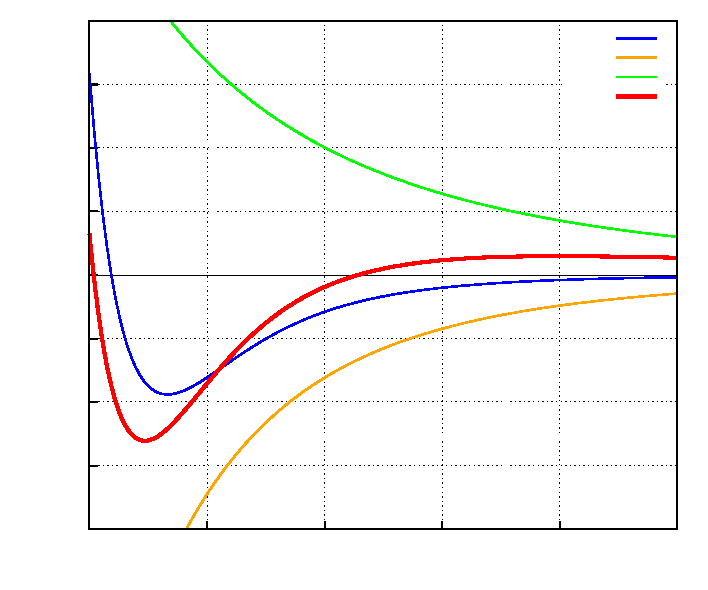
\includegraphics{n3_benzene_pes}}%
    \gplfronttext
  \end{picture}%
\endgroup

    \caption{Potential energy surface of \ntm and a benzene ring.}
    \label{fig:n3_benzene_pes}
\end{figure}
%
As we can notice, the magnitude of the induction and the electrostatic potentials are
comparable. In the long range regime, the Coulomb interaction, decaying as $1/r$, is stronger
and the total potential is repulsive.
Nevertheless, this is just a toy model and does not provide quantitative results.
Note that the charges used on the benzene wer arbitrarily set to $-0.1$ on the carbon atoms
and to $+0.1$ on the hydrogen atoms.
Moreover, consider that the ILJ parameters used are not optimized for the interaction 
between \ntm and a benzene ring.\\

\subsubsection{Forces}
Accounting for the above considerations, we expect both the electrostatic and induction forces
to be of comparable magnitude, but pointing in opposing directions.
Therefore, by checking that the induction forces are within the same range of values than
the Coulomb forces, and that their direction corresponds to their physical interpretation,
we can reasonably think that there is no mistake in the implementation.\\
In \Cref{tab:forces_benzene_att} we can see the values of the $z$ component of the forces acting
on the benzene molecule due to the azide anion, when placed at a distance $R=4$ \AA.
Note that the $z$ component is the most important one as it tells us if the two fragments
are attracting or repelling each other.
Only values for symmetry-unique atoms of the benzene molecule are shown in
\Cref{tab:forces_benzene_att}, with the number of repetition in parenthesis.
A negative sign means repulsion, i.e. the force on the (benzene) atom is directed in the
opposite direction with respect to the position of the azide anion, and viceversa.
The only negative forces are observed for the carbon atoms, and this is due to their negative
charges repelled by the negative charges on the external nitrogen atoms.
Notice that all induction forces are positive (i.e. pulling the benzene molecule towards
the \ntm) as they should be, because the induction potential always lowers the energy and
thus attracts the fragments.
In the last element of the last row of \Cref{tab:forces_benzene_att} we see that
the total force on the benzene molecule is positive, i.e. in the direction of the \ntm.
This is indeed what we expect by inspecting \Cref{fig:n3_benzene_pes}, as at $R=4$ \AA\ the
(total) potential is in the attractive region.\\
%
\begin{table}
    \captionsetup{width=\textwidth}
    \centering
    \caption{$z$ component of the force on the benzene due to the azide anion
    at interfragment distance of $R=4$ \AA. Values are given in $10\times$J/mol.}
    \begin{tabular}{ccccc}
    \toprule
    atom label  & vdw     & electrostatic & induction & total \\
    \midrule
    (2x)C4    & $+50.85$  & $-645.26$     & $+179.76$ & $-414.65$ \\
    (4x)C5    & $+16.91$  & $-675.81$     & $+198.39$ & $-460.51$ \\
    (2x)H10   & $+18.04$  & $+483.32$     & $+31.94$  & $+533.30$ \\
    (4x)H11   & $+20.60$  & $+534.16$     & $+39.49$  & $+594.25$ \\
    \midrule
    benzene   & $+287.82$ & $-890.48$     & $1374.92$ & $+772.26$ \\
    \bottomrule
    \end{tabular}
    \label{tab:forces_benzene_att}
\end{table}
%
We repeat the same calculation, but now for an interfragment distance of $R=3.25$ \AA, thus
in the repulsive region of the potential.
Indeed, we observe from \Cref{tab:forces_benzene_rep} that the total force is now pushing
the benzene molecule away from the \ntm ion.
In particular we notice in the first column the strong repulsion due to the ILJ potential.
The contributions from both electrostatic and induction did not change direction, obviously,
but increased in magnitude. Again, this is behavior corresponds with the PES depicted in
\Cref{fig:n3_benzene_pes}.
%
\begin{table}
    \captionsetup{width=\textwidth}
    \centering
    \caption{$z$ component of the force on the benzene due to the azide anion
    at interfragment distance of $R=3.25$ \AA. Values are given in $10\times$J/mol.}
    \begin{tabular}{ccccc}
    \toprule
    atom label  & vdw      & electrostatic & induction & total \\
    \midrule
    (2x)C4    & $-299.04$  & $-855.22$     & $+388.56$ & $-765.70$ \\
    (4x)C5    & $-889.79$  & $-936.38$     & $+471.21$ & $-1354.96$ \\
    (2x)H10   & $+43.21$   & $+580.89$     & $+56.78$  & $+680.88$ \\
    (4x)H11   & $+13.34$   & $+689.67$     & $+81.60$  & $+784.61$ \\
    \midrule
    benzene   & $-4017.46$ & $-1535.54$    & $3101.92$ & $-2451.04$ \\
    \bottomrule
    \end{tabular}
    \label{tab:forces_benzene_rep}
\end{table}
%

\subsubsection{Virial and stress tensor}


\end{document}
